%----------------------------------------------------------------------------
\chapter{Kiértékelés valós adatokon}\label{chapter:kiertekelesvalos}
%----------------------------------------------------------------------------

Ez a fejezet mutatja be a Bayes-döntés alapján diszkretizáló algoritmus használhatóságát valós adatokon. A valós adatok vérképekből származnak, azt vizsgálva, hogyan alkalmazható az eljárás labordiagnosztikai paraméterek diszkretizálására.

\section{Adatsor}
A kísérletek során rendelkezésre állt a Semmelweis Egyetem Általános Orvostudományi Karának Laboratóriumi Medicina Intézetéből származó vérképeket tartalmazó adatbázis. Az adatbázis rekordjai tartalmazzák többek között a következő adatokat: a sor azonosítója, a páciens azonosítója visszafejthetetlenül egyirányúan titkosítva, így nem beazonosítható, de az egy pácienshez tartozó mérések összepárosíthatók, a páciens neme, életkora, a vérképelemzés kérésének időpontja, a mért paraméter kódja, a mérés eredménye és a mért paraméter referencia tartománya.

Az adatbázisban tartalmazott adatokban előfordulhat mérési hiba. Az adott időszakban a laboratóriumban végzett mérések nagy része megtalálható benne, így egy vizsgálat során több mért paraméter mindegyike szerepel az adatbázisban.

\begin{figure}[htp]
    \centering
    \includegraphics[width=8cm]{figures/cardio/cardio_start.png}
    \caption{Az esettanulmányban elkészült háló részgráfja}
    \label{fig:cardio_start}
\end{figure}

A kísérletekhez Fuster-Parra et al. \cite{fuster2016bayesian} esettanulmánya szolgáltatta az alapot. Ebben Bayes-háló modellt építenek a szív- és érrendszeri betegségek kockázatának feltárására. Az általuk kialakított háló részgráfja a \ref{fig:cardio_start}. ábrán látható. A \emph{Kor} a páciens kora, \emph{Nem} a neme, \emph{koleszterin, trigliceridek és vércukor} pedig a laboratóriumi paraméterek. Az eredeti háló ezeken kívül tartalmazza a páciensről, hogy dohányzik-e, végez-e testmozgást, a testtömeg indexét, derékbőségét, vérnyomását, van-e metabolikus szindrómája. Ezek mellett a Framingham-REGICOR pontszámát, amely a Framingham-REGICOR egyenlet alapján a szív-és érrendszeri betegség kockázatát adja meg \cite{amor2017prediction}, valamint az "elvesztett évek számát", mely a kiszámolt szív kor és a valódi kor különbsége.

Ilyen típusú adatokat, valamint a kiszámolásukhoz szükséges adatokat nem tartalmazza a rendelkezésre álló adatbázis, így ezek nem vesznek részt a kísérletben. A rendelkezésre álló változókból az eredeti feszített részgráfja lett képezve, ez volt a kísérletek során felhasználva. A kimaradt változókon keresztüli feltételes függőségek ebben a modellben nem szerepelnek.

Az adatbázisban egy rekordban egyetlen paraméter szerepel. A koleszterinhez tartozó \emph{HDLC} kódú adatokból 177 473, a vércukorszinthez tartozó \emph{GLU} kódú adatokból 269 657, valamint a trigliceridekhez tartozó \emph{TGL} kódú adatokból 264 209 pácienshez rendeltek mérést. Páciensenként az első adatpont lett kiválasztva, és azok maradtak, akiknek mindhárom laboratóriumi paraméterét  megmérték. Ez 119 477 páciensre igaz, amiből látható, hogy ha koleszterin szint mérést kértek valakinél, annál 67\% eséllyel mindkét másik paramétert is mérték.

Fennáll az a hibalehetőség, hogy az eldobott adatok nem véletlenszerűek, hanem összefüggés van valamelyik értékkel. Lehetséges például, hogy az alacsony koleszterinszint eredmény után a másik kettőre kisebb eséllyel tesztelnek, ezért a szűrt adatsorban az átlagos koleszterinszint magasabb lesz. Ez egy MNAR (Missing Not At Random) típusú hiányzás \cite{rubin1976inference}.

\begin{table}[htp]\centering
\begin{tabular}{lc}
    Laboratóriumi paraméter & Referencia tartomány \\ \hline
    Koleszterin             & 0.9 – 1.5            \\
    Trigliceridek           & 0.5 – 2.0            \\
    Vércukor                & 3.9 – 5.8
    \end{tabular}
    \caption{A jelenleg használt referencia tartomány a vizsgált laboratóriumi paraméterekhez.}
    \label{tab:cardio_referencia}
\end{table}

Az így kapott adatsorban szerepel a páciens életkora, neme, valamint a hozzá tartozó koleszterinszint, trigliceridek mennyisége és a vércukor szintje a vérképe alapján. Ebből a nem változó diszkrét, a többi folytonos. A laboratóriumi paraméterek referencia tartománya, amely az eredeti adatbázisban szerepelt, a \ref{tab:cardio_referencia}. táblázatban látható.

\section{Futtatás}
A változók elnevezése az ábécé betűivel a kor, nem, koleszterin, trigliceridek, vércukor sorrendben történt. Ez alapján a kiindulási gráf topológiai sorrendje \emph{B, A, C, E, D}. Az A és C felcserélhető, a többi helye meghatározott.

A teljes adatsoron így futtatva se az \emph{B, A, C, E, D}, se a \emph{B, C, A, E, D} sorrendre nem határozott meg diszkretizációs elvet, ezeknél az alapértelmezett értékeket adta vissza, valamint egyetlen él sem lett a k2 által tanult gráfba felvéve. Ilyen akkor történik, amikor a k2 algoritmusban minden változó kihagyása jobb, mint kettő összekötése. Az értékeket a kezdeti diszkretizáció után vizsgálva látható, hogy szinte minden érték egyforma. Ennek oka, hogy a kezdeti diszkretizáció egyenlő hosszú intervallumok alapján történik, az adatsorban pedig sok a kiugró érték.

A kezdeti diszkretizáció módosítását támogatja az elkészült csomag, használható az egyenlő mintaszámú diszkretizáció a nem egyenletes eloszlású adatokon, amilyen ebben az esetben is szerepel.

Így futtatva az algoritmust \emph{MemoryError} exception keletkezik. Ennek oka, hogy a dinamikus programozással megoldott algoritmus egy $n^{2}$ méretű tömböket használ a részeredmények tárolására. E a 119 477 elemű adatsorhoz 100 GB feletti tárterületet igényel. Ezért az implementált algoritmus nem tud ekkora mennyiségű adaton dolgozni.

\begin{table}[htp]\centering
    \begin{tabular}{lcc}
    Változó       & Referencia tartomány & Ismert sorrend    \\ \hline
    Kor           & -                    & 34.36, 48.61      \\
    Koleszterin   & 0.9, 1.5             & 1.29, 1.69, 3.33  \\
    Trigliceridek & 0.5, 2.0             & 1.08, 14.57       \\
    Vércukor      & 3.9, 5.8             & 4.65, 5.35, 33.95
    \end{tabular}
    \caption{A diszkretizációs határok a referencia tartományok szerint és az algoritmus ismert topológiai sorrenden történő futtatásával.}
    \label{tab:cardio_kisebb_adat}
\end{table}

Erre megoldási lehetőség, hogy az adatoknak kis részén fut az eljárás. Ehhez véletlenszerűen kiválasztható az adatsor $\frac{1}{100}$-ad része. A kisebb mennyiségen futtatva kapott eredményt a \ref{tab:cardio_kisebb_adat}. táblázat mutatja. Az eltérések rendkívül nagyok, az algoritmus pedig nagyon nagy számokat is ajánl határnak. Ennek oka a már felfedezett kiugró értékek az adatsorban, melyek mérési vagy beviteli hibákból adódhatnak.

\begin{figure}[htp]
    \centering
    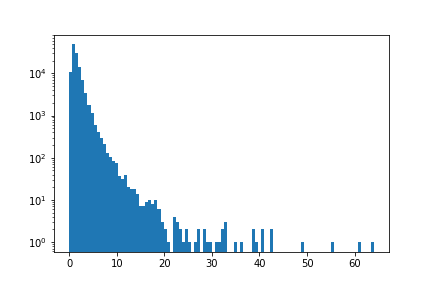
\includegraphics[width=8cm]{figures/TGL_hist.png}
    \caption{A trigliceridek hisztogramja logaritmikus skálán}
    \label{fig:cardio_tgl_hist}
\end{figure}

A trigliceridek változó értékeinek 100 vödörbe osztott hisztogramja a \ref{fig:cardio_tgl_hist}. ábrán található. Az \emph{y} tengely skálázása logaritmikus, így láthatók a kis értékek is. A 18-as értékig minden vödörbe legalább 10 adatpont esett, utána előfordulnak 0 és 1 adatot tartalmazó vödrök. Ilyen mennyiségű adatnál ezek kiugró értékeknek számítanak.

Ezért minden folytonos változó eredeti adatainak felső és alsó 5 percentilise eltávolítható az adatsorból, így a hibák nem kerülnek az algoritmus tanító adataiba. Az eredeti adatsorban így 80 462 adatpont marad, amely a tanításhoz így is túl sok, úgyhogy az adatoknak továbbra is 1\% adódik tanító adatnak.

Az ismert topológiai sorrend mellett a kísérlet elvégezhető az információelméleti alapon kiszámolt sorrenden is. Ekkor a sorrend \emph{B, C, D, E, A}-nak adódott.

\begin{table}[htp]\centering
\begin{tabular}{lccc}
    Változó       & Referencia tartomány & Ismert sorrend & Kezdeti sorrend \\ \hline
    Kor           & -                    & 39.18, 60.35   & 48.09           \\
    Koleszterin   & 0.9, 1.5             & 1.31, 1.58     & 1.15, 1.69      \\
    Trigliceridek & 0.5, 2.0             & 0.89, 1.60     & 0.69, 1.25      \\
    Vércukor      & 3.9, 5.8             & 4.75, 5.45     & 4.05, 5.25
    \end{tabular}
    \caption{A diszkretizációs határok a referencia tartományok szerint és az algoritmus ismert topológiai sorrenden történő futtatásával, kiugró értékek eltávolítása után.}
    \label{tab:cardio_kiugro_ertek}
\end{table}

\begin{figure}[htp]
    \centering
    \includegraphics[width=8cm]{figures/cardio/cardio_ismert.png}
    \caption{A tanult Bayes-háló az algoritmus ismert topológiai sorrenden történő futtatásával, kiugró értékek eltávolítása után.}
    \label{fig:cardio_kiugro_ertek}
\end{figure}

\begin{figure}[htp]
    \centering
    \includegraphics[width=8cm]{figures/cardio/cardio_kezdeti.png}
    \caption{A tanult Bayes-háló az algoritmus ismert topológiai sorrenden történő futtatásával, kiugró értékek eltávolítása után.}
    \label{fig:cardio_kiugro_ertek_kezdeti}
\end{figure}

Az így futtatott algoritmus a \ref{tab:cardio_kiugro_ertek}. táblázatban található referencia tartományokat állapítja meg. Az ismert sorrenddel futtatott algoritmus a \ref{fig:cardio_kiugro_ertek}. ábrán látható, a számolt kezdeti sorrenddel futtatott a \ref{fig:cardio_kiugro_ertek_kezdeti}. ábrán látható Bayes-hálót építi fel.

